\Def Пусть задано $S \subset \R^2, |S| < \infty$, тогда выпуклой оболочкой называют выпуклый многоугольник минимальной площади,
содержащий внутри себя $S$.

\begin{figure}[h]
    \centering
    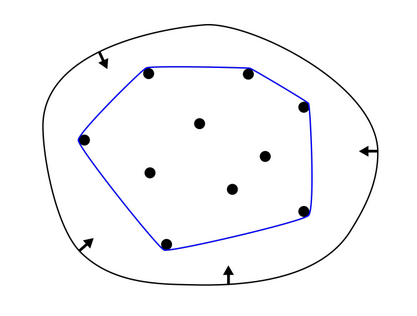
\includegraphics[scale = 0.4]{pix/convex_hull.png}
\end{figure}

\textbf{Алгоритм Джарвиса.} 
\begin{enumerate}
    \item Пусть $P_0$ — самая левая (из них самая нижняя) точка.
    \item Введем $P_1$ — точка с минимальным углом относительно между осью $OY$ и $P_0P_1$.
    \item $\forall i > 1$ точка $P_i$ определяется как точка с максимальным углом $\angle P_{i-2}P_{i-1}P_i$
\end{enumerate}

\begin{figure}[h]
    \centering
    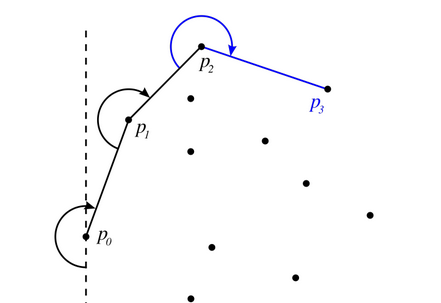
\includegraphics[scale = 0.8]{pix/convex_hull_Jarvis.png}
\end{figure}

\textbf{Aсимптотика:} Поиск $P_0$, $P_1$ занимает $\mathcal{O}(n)$ времени, так как это наивный перебор. Поиск $P_i$ составит в свою очередь аналогично $\mathcal{O}(n)$, так как надо перебрать все точки. Пусть $h$ — число точек в выпуклой оболочке, тогда время работы составит $\Theta(nh) = \mathcal{O}(n^2)$.

\pagebreak